\documentclass[twocolumn,10pt]{ltjsarticle}

\usepackage[top=20mm,bottom=20mm,left=25mm,right=25mm,columnsep=10mm]{geometry}
\usepackage[haranoaji,nfssonly]{luatexja-preset}
\usepackage{graphicx}

\title{【調査】プロキシサーバのログを用いたRATの検知}
\author{山下 尚彦}
\date{\today}

\begin{document}
\maketitle

\section{はじめに}
特定の組織をターゲットとした標的型攻撃の多くは, 攻撃対象の端末を遠隔で操作できる
Remote Access Trojan(RAT)が用いられ, その通信の多くはHTTPプロトコルが使われており, 
通信先や特徴的な通信パターンが判明していない限り検知することは困難である. 
そのため, 従来のRAT検知手法では機械学習などを用いたパターンマッチングによる検知が主流であった. \par
三村らの研究\cite{三村守2016http}では従来の手法とは違い, パターンマッチングを用いないRAT検知手法と
通信先のブラックリストを併用したHTTPプロトコルベースの通信挙動によるRAT検知システムの運用構想を提案している. 
実際に運用されているネットワークでの実験を行った結果, RATによる外部の通信は発生しなかったため, 
誤検知はしなかった. しかし, 不正な通信の検知に関しては新たな知見を得られることはできなかった. 

\section{関連研究}
三村らは, プロキシサーバのログからクライアントのアドレス, 通信先のアドレス及びリクエスト数を用い, 
クライアントと共通するサーバに着目してグループに分類し, 疑わしいドメインを検出する手法を提案した
Tranらの研究\cite{tran2014supplementary}を元にRAT検知システムを構築した. 
この関連研究ではDNSのログ, プロキシサーバのログなどを使用し, 内部ホストの訪問履歴と
そのUser Agentから組織全体の希少な訪問サイト, User Agentの傾向, ドメインの類似性などを
教師なし学習で分析し, 通常状態と比較することで異常なドメインから検出することができたが, 
DNSサーバなどのログも必要となったり, ドメイン情報やブラックリストなどの外部情報も必要となることが
課題である. \par
三村らは, 教師あり学習モデルに着目し, さらにプロキシサーバのログのみを用いてRATを検知しようと試みた. 

\section{提案手法}
\subsection{前提条件}
プロキシサーバのログの内, 以下の情報を使用する. 

\begin{itemize}
    \item タイムスタンプ
    \item HTTPリクエストの内容(メソッド, URL, User Agent)
    \item HTTPレスポンスステータスコード
    \item HTTPレスポンスサイズ
\end{itemize}

これらの情報はプロキシサーバの標準的なログのフォーマットであるため, 多くのプロキシサーバで取得可能である. 
このログから, HTTPレスポンスステータスコードが成功(2xx)の行を対象としてURLに含まれるホストごとに
適切な行数のログを抽出する. 

\subsection{特徴ベクトルと学習}
前述した情報を含んだログファイルからステータスコードが成功した行のログを適切な行数抽出し, 
それぞれの項目の頻度から以下の特徴ベクトルを作成する. 

\begin{itemize}
    \item 最頻出の受信サイズ
    \item 最頻出の受信サイズの数
    \item 最頻出のリクエストの間隔
    \item 最頻出のリクエストの間隔の数
    \item 最頻出のpathの長さ
    \item 最頻出のpathの長さの数
    \item POSTメソッドの数
    \item User Agentの長さ
\end{itemize}

作成した特徴ベクトルがRATによる通信であればRATの種類, それ以外は正常な通信のラベルを付与し学習させる. 
学習にはSupport Vector Machine(SVM)とRandom Forests(RF)を教師あり学習モデルとして利用し, 
未知のデータの予測させる. 

\section{実験}
\subsection{実験環境}
三村らは3章で提案した手法を実際に運用されているネットワークに用いて実験を行った. 
このネットワークを利用するユーザは25万人程度いて, 主にWebやメールなどが主な用途である. 
そのネットワーク内で1ヶ月間, 事前に学習させたRAT検知システムを稼働させた. 学習に用いたデータは, 
2015年に大規模なサイバー攻撃を受けた組織の1日分のプロキシサーバのログで, 通常のHTTP通信以外に
2種類のRATによる遠隔操作された通信が記録されていた. 

\subsection{実験結果}
以下の\textbf{表\ref{table:result}}は実験結果である. 表のRT, FV, DCはそれぞれ1時間分のログにおいて, 
予測モジュールで処理するのに要した時間, 生成された特徴ベクトルの数, RATと判定された数を示す. 

\begin{table}[htb]
    \caption{実験結果}
    \label{table:result}
    \centering
    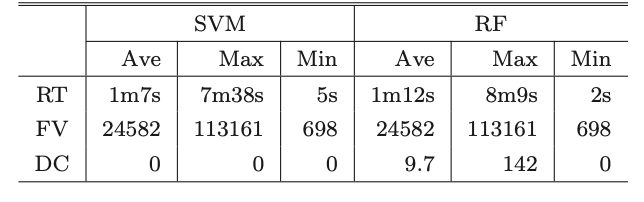
\includegraphics[width=6cm]{images/【調査】プロキシサーバのログを用いたRATの検知/result.png}
\end{table}

1時間分のログを処理する時間はSVMとRF双方において平均1分程度, 最大でも10分と比較的短時間で処理することが可能であった. 
また, 生成された特徴ベクトルの数は時間帯によってネットワークを利用するユーザが異なるため, それに比例して大きな差があった. 
RATと判定された数は, SVMでは0件, RFでは一時間平均10件, 最大142件検知された. 
しかし, 実験環境ではRATによる外部の通信は発生していなかったため, RFによる検知はすべて誤検知である. 
これは同一の長さの通信を短時間に頻繁に繰り返すという特徴のあるRATと正常な通信を区別することができなかったためであると考えられる. 

\section{考察}
実験期間中, RATによる不正な通信は確認できなかったため, RATの検知について知見は得られなかった. 
同様に, 学習させたログに含まれていたRATとは違う未知のRATによる通信について検知することができるかも検証する必要がある. 
しかし, 正常な通信を不正な通信と誤った判定をすることはSVMでは全く発生せず, RFを用いた方法でもやや発生する程度あるため, 
実運用のネットワークに適用することは可能であると三村らは結論づけた. 

\section{おわりに}
三村らは, プロキシサーバのログからRATの不正な通信を学習させ, 実際のネットワークで実験を行った. 
RAT検知システムを稼働させていた1ヶ月では, RATの不正な通信が発生しなかったため, RATを検知する点においては
評価することができないが, 正常な通信を誤検知する回数は許容できる範囲であったと考えられる. \par
私の研究では, ネットワーク内のトラフィックデータ全てを監視する必要があったため, 三村らの手法のように
プロキシサーバ等のログデータからボットネットの周期性を判定することで, 解析に必要なデータサイズを減らすことが可能だと思われる. 
また, 常時ネットワークを監視する必要がないため, 実運用のネットワークに適用しやすいだろう. 

\bibliographystyle{junsrt}
\bibliography{DB}
\end{document}